% !TEX root = RKWard_paper.tex
\section{Background and motivation}
\label{background}
In mid 1993 Ihaka and Gentleman published initial efforts on the computing
language and programming environment \proglang{R} on the \emph{s-news} mailing list. Ambitions for
this project were to develop an \proglang{S}-like language without inheriting memory
and performance issues. The source code of \proglang{R} was finally released in 1995, and 
since 1997 development has evolved under the umbrella of the \proglang{R} 
Development Core Team \citep{RDCT2001, RDCT2010, Ihaka_Gentlemen_1993}.
\proglang{R} does not include an advanced cross-platform graphical user interface (GUI) as known from other
statistical software packages. However, \proglang{R} includes tools for building GUIs
mainly based on \proglang{Tcl/Tk} \citep{Dalgaard2001, Dalgaard2002}. Meanwhile a
plethora of \proglang{R} GUIs have emerged \citep[see][for a comprehensive list]{RGUI}. In 2005 John Fox released version 1.0 of \proglang{R} Commander \citep[package \pkg{Rcmdr}]{Fox2005}, which
can be considered a milestone in \proglang{R} GUI development; it was the first GUI
implementation that was able to make statistical tests,
plots and data manipulation easily accessible for \proglang{R} novices.
John Fox stated that \pkg{Rcmdr}'s target was to provide
functionality for basic-statistical courses, though the features have increased over
time beyond this \citep{Fox2005, Fox2007}. In November 2002 Thomas Friedrichsmeier
started the \pkg{RKWard} open-source software project with the goal to create a GUI for
\proglang{R} based on \pkg{KDE}\footnote{
  \pkg{KDE} is a desktop environment and software collection based on \pkg{Qt} (http://www.kde.org/).
  In the context of this paper, the term \pkg{KDE} is primarily used to refer to the programming library and
  runtime environment of \pkg{KDE}, rather than the complete software collection. For an introduction to
  \pkg{KDE} as a programming library, see \cite{Faure2000}.
} and \pkg{Qt}\footnote{
  \pkg{Qt} is a \proglang{C++}-based cross-platform programming library with a focus on GUI development
  \citep{BlanchetteSummerfield2008}. Online documentation is available at http://qt.nokia.com/.
} technologies.

The scope of \pkg{RKWard} is deliberately broad, targeting both \proglang{R} novices and experts.
For the first group, the aim is to allow any person with knowledge on
statistical procedures to start using \pkg{RKWard} for their everyday work 
without having to learn anything about the \proglang{R} programming language,
at least initially. At the same time, \pkg{RKWard} tries to support users who want to learn and
exploit the full flexibility of the \proglang{R} language for automating or customizing
an analysis. At the other end of the learning curve, \pkg{RKWard} provides advanced integrated development environment (IDE)
features to \proglang{R} experts to assist in writing \proglang{R} scripts. Yet, the idea
is that \proglang{R} experts too will benefit from the availability of task-oriented GUI
dialogs, such as when exploring an unfamiliar type of analysis
or by allowing to implement routinely performed tasks as a GUI element. In
addition, many features like the integrated data editor and the plot preview 
will be useful to \proglang{R} novices and \proglang{R} experts alike in their everyday work
(see Section~\ref{sec:user_interface}).

\pkg{RKWard} provides a high level of transparency about the steps that are needed to
perform any supported task in \proglang{R}, in order to make it easy for the user to see
complete codes for all GUI actions\footnote{
  This distinguishes \pkg{RKWard} from \proglang{R} GUIs such as \pkg{Red-R} (http://www.red-r.org/), which 
  specifically aims to hide the complexities of the \proglang{R} programming language, following the concept of visual data-flow 
  programming \citep{Sutherland1966}. In contrast, \pkg{RKWard} limits itself to generate \proglang{R} code from GUI settings.
}. In doing so, \pkg{RKWard} deliberately generates
comparatively verbose code. It avoids wrapping complex sequences of data
manipulation or analysis into custom high-level \proglang{R} functions. The task of
providing high-level functions is logically independent of the development of the
GUI frontend, and should best be addressed in dedicated \proglang{R} packages, where necessary.
This approach allows to make better use of the modular design of \proglang{R}, avoids
locking-in users to a specific GUI application, and provides them with more options for
customizing the generated code patterns.

While \pkg{RKWard} tries to address users wishing to learn \proglang{R}, it is specifically not
designed as a teaching tool -- such as \pkg{Rcmdr} \citep{Fox2005} or \pkg{TeachingDemos} \citep{TeachingDemos2010} -- but as
a productive tool. Since its incarnation \pkg{RKWard} has gained acceptance for usage in peer-reviewed 
publications \citep{Zou2008, Zou2009, Rugg-Gunn2010, Yang2011, Roediger2011, Roediger_VS}.
Dialogs for statistical procedures in \pkg{RKWard} do not
necessarily show a one-to-one correspondence to the underlying steps in \proglang{R}, but are
rather oriented at statistical tasks. Furthermore, \pkg{RKWard} does not impose
artificial limitations on how users can work with the application. For example,
the user is not limited to using only one \code{data.frame} or one model at a
time.

\pkg{RKWard} is designed to allow users to create custom GUI dialogs as plugins, requiring relatively
little programming knowledge. In essence, \pkg{RKWard} plugins consist of an XML file describing
the dialog layout, and \proglang{ECMAScript} code which generates \proglang{R} code from the settings
made in the GUI. Most of the data handling functionality in \pkg{RKWard} is implemented as plugins
(see Section~\ref{sec:analyzing_data}), and many of these plugins have originated as user contributions.
Since version 0.5.5, \pkg{RKWard} also provides support for downloading user contributed ``plugin packs'',
which are not included in the official \pkg{RKWard} releases. Details on the definition of plugins,
and a commented example can be found in the technical supplement to this article.

\pkg{RKWard} is licensed under the terms of the GNU General Public License\footnote{http://www.gnu.org/licenses/gpl.html} Version 2
or higher. However, due to its dependencies, \pkg{RKWard} binaries are effectively
distributable only under the terms of Version 2 of the license. Parts of the documentation are available under the
GNU Free Documentation License\footnote{http://www.gnu.org/licenses/fdl.html}. While the project remains in constant development, a growing
number of users employs \pkg{RKWard} in productive scenarios. The source code,
selected binaries and documentation is hosted at SourceForge
(\url{http://rkward.sourceforge.net/}). Selected key milestones of the development of \pkg{RKWard} are
visualized in Figure~\ref{fig:timeline}.

In this paper we will give an overview over the installation process (Section~\ref{sec:installing_starting_RKWard}), the main GUI elements and
features of \pkg{RKWard} (Section~\ref{sec:user_interface}), and closing by a short example 
of a simple \pkg{RKWard} session (Section~\ref{sec:using_RKWard}). For readers interested in the technical
design, and reasons for certain design decisions, a technical supplement to this article
is available.

\begin{figure}[t!]
 \centering
 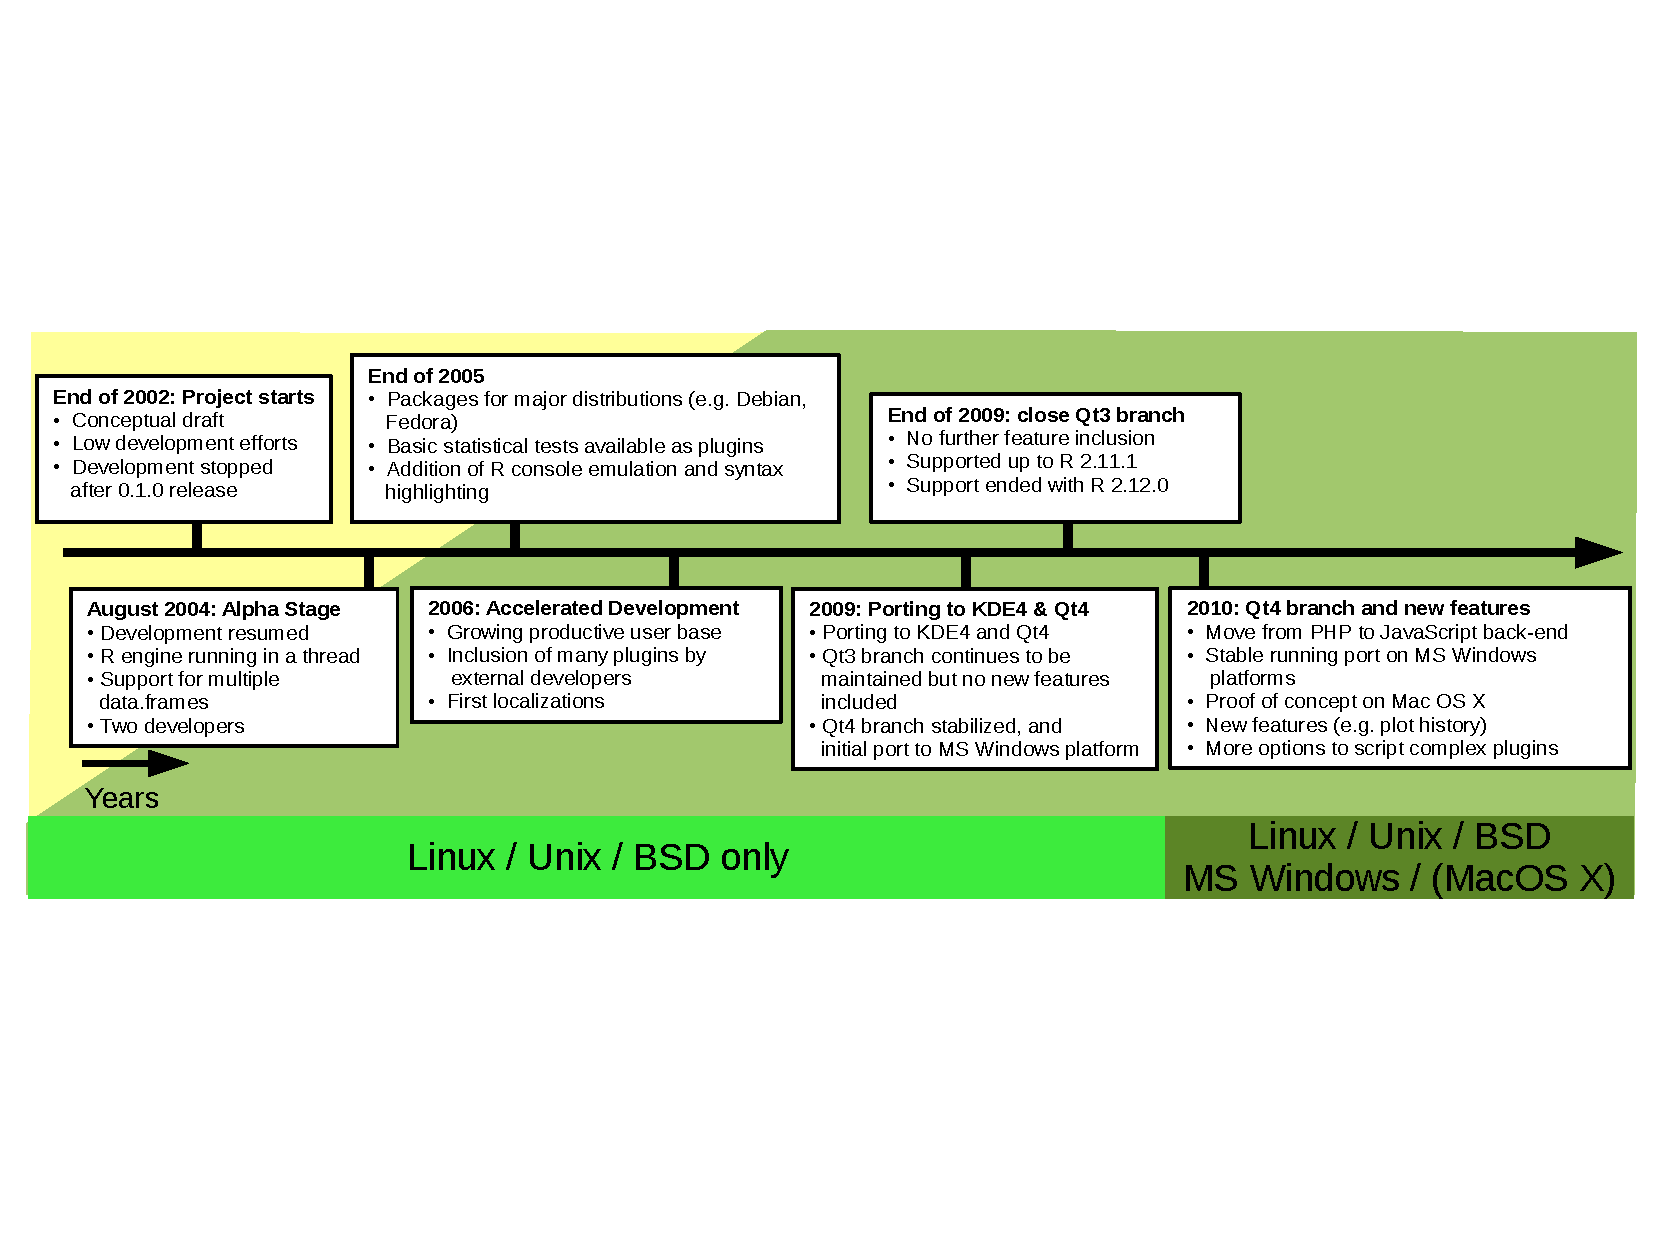
\includegraphics[clip=true,trim=0cm 5.7cm 0cm 5.7cm,width=15.4cm]{./figures/timeline.pdf}
 \caption{Timeline of important development milestones and changes in \pkg{RKWard}.
          Time is presented on an arbitrary scale. Here \pkg{Qt}3 and \pkg{Qt}4 refers to the 3.x and
          4.x versions of the \pkg{Qt} libraries, respectively and \pkg{KDE}4 refers to the
          4.x version of the \pkg{KDE} libraries.}
 \label{fig:timeline}
\end{figure}
